% Fit check for every figure and table, on a page that emulates the Springer LNCS layout:
% 10 pt Computer Modern, text area 122 mm x 193 mm, captions 9 pt with bold "Fig. 1." / "Table 1." labels.
% In the real paper use \documentclass[runningheads]{llncs} instead; it sets all of this itself.
\documentclass[10pt]{article}
\usepackage[a4paper,textwidth=122mm,textheight=193mm,centering]{geometry}
\usepackage[T1]{fontenc}
\usepackage{graphicx,booktabs,array,amssymb,tabularx,makecell}
\usepackage[font=small,labelfont=bf,labelsep=period]{caption}
\renewcommand{\figurename}{Fig.}
\graphicspath{{../figures/}}
\begin{document}
\section*{LNCS fit check: paper (Figs. 1--3, Tables 1--8)}
Each float below is included exactly as in the paper. An overfull box warning in the log means a float is wider than the 122 mm text area.

\begin{figure}[tb]
\centering
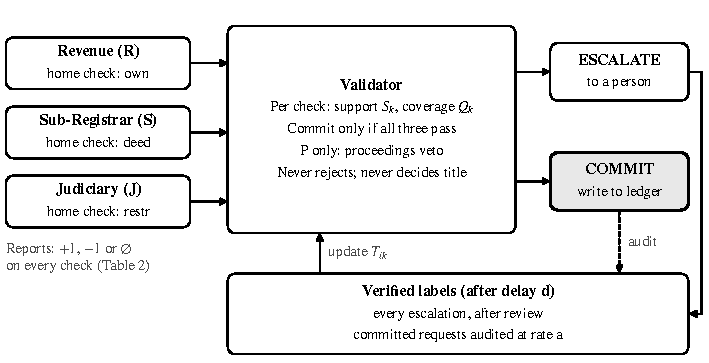
\includegraphics[width=\textwidth]{fig1_system.pdf}
\caption{Validation loop. Three offices report on three checks, the validator commits a request only when all three checks pass and otherwise escalates it, and verified labels update trust.}
\label{fig:system}
\end{figure}

% Auto-generated by paper_assets/build_assets.py from saved results -- do not edit numbers by hand.
% Preamble needs: \usepackage{booktabs,array,tabularx,makecell}
\begin{table}[tb]
\centering
\caption{Comparison with related work}\label{tab:related}
\footnotesize
\setlength{\tabcolsep}{2pt}
\renewcommand{\arraystretch}{1.1}
\begin{tabularx}{\textwidth}{@{}>{\raggedright\arraybackslash}p{2.0cm}*{7}{>{\raggedright\arraybackslash}X}@{}}
\toprule
Work & Land records & Multi-source & Per-claim authority & Learned trust & Pre-commit conflict check & Escalates & Ground truth \\
\midrule
Thakur et al. [1] & yes & yes (nodes) & no & no & no (deferred) & manual & no \\
Soner et al. [5]$^\dagger$ & yes & yes & ? & ? & ? & ? & ? \\
Shuaib et al. [6]$^\dagger$ & yes & ? & ? & ? & ? & ? & ? \\
Sahai, Pandey [7]$^\dagger$ & yes & ? & ? & ? & ? & ? & ? \\
Khanna et al. [15]$^\ddagger$ & yes & yes (6 roles) & role-based & n.s. & n.s. & n.s. & n.s. \\
Chainlink [10] & no & yes (nodes) & no & reput. & aggreg. & no & no \\
Truth discovery [13] & no & yes & no & yes (unsup.) & yes & no & --- \\
DecenTruth [14]$^\ddagger$ & no & yes & no & yes (unsup.) & yes & n.s. & sim. \\
This work & synthetic & yes (3) & yes & yes (labels) & yes & yes & yes \\
\bottomrule
\end{tabularx}
\par\smallskip
\parbox{\textwidth}{\scriptsize $^\dagger$ Full text not yet read; ? = not determined. $^\ddagger$ Compared at abstract level only. n.s. = not stated in the abstract; unsup. = estimated without labels; reput. = reputation; aggreg. = aggregation of node reports; sim. = simulation; --- = not applicable to a survey.}
\end{table}

% Auto-generated by paper_assets/build_assets.py from saved results -- do not edit numbers by hand.
% Preamble needs: \usepackage{booktabs,array,tabularx,makecell}
\begin{table}[tb]
\centering
\caption{Claim-specific authority $A(i,k)$ (modelling assumption)}\label{tab:authority}
\small
\setlength{\tabcolsep}{3pt}
\renewcommand{\arraystretch}{1.1}
\begin{tabular}{@{}lccc@{}}
\toprule
Check & Revenue & Sub-Registrar & Judiciary \\
\midrule
own & 1.0 & 0.6 & 0.4 \\
deed & 0.6 & 1.0 & 0.4 \\
restr & 0.2 & 0.2 & 1.0 \\
\bottomrule
\end{tabular}
\end{table}

% Auto-generated by paper_assets/build_assets.py from saved results -- do not edit numbers by hand.
% Preamble needs: \usepackage{booktabs,array,tabularx,makecell}
\begin{table}[tb]
\centering
\caption{Worked example: request 123 in S5a, seed 1, with a pending proceeding visible only to the Judiciary}\label{tab:example}
\footnotesize
\setlength{\tabcolsep}{3pt}
\renewcommand{\arraystretch}{1.1}
\begin{tabularx}{\textwidth}{@{}lcl>{\raggedright\arraybackslash}Xl@{}}
\toprule
Mechanism & \makecell{Support for \\ `clear' on restr} & Decision & Reason code & Outcome \\
\midrule
B1 Majority & 2 of 3 clear & COMMIT & --- & false commit \\
B2 Authority-only & 0.286 & ESCALATE & restr: low support & escalated \\
B3 Trust-only & 0.666 & COMMIT & --- & false commit \\
P$-$V Hybrid & 0.285 & ESCALATE & restr: low support & escalated \\
P Hybrid + veto & veto first & ESCALATE & veto: proceeding reported & escalated \\
\bottomrule
\end{tabularx}
\par\smallskip
\parbox{\textwidth}{\scriptsize Truth: own pass, deed pass, restr pending (request invalid). Reports (own, deed, restr): R: +1 +1 +1; S: $-$1 +1 +1; J: +1 +1 $-$1. Trust under ideal feedback at that point: R, S and J on restr $\approx$ 1.00; $\theta$ = 0.65.}
\end{table}

\clearpage
% Auto-generated by paper_assets/build_assets.py from saved results -- do not edit numbers by hand.
% Preamble needs: \usepackage{booktabs,array,tabularx,makecell}
\begin{table}[tb]
\centering
\caption{Scenarios; each changes one setting from S1}\label{tab:scenarios}
\footnotesize
\setlength{\tabcolsep}{3pt}
\renewcommand{\arraystretch}{1.1}
\begin{tabularx}{\textwidth}{@{}l>{\raggedright\arraybackslash}Xc@{}}
\toprule
Scenario & Change from S1 & RQ \\
\midrule
S1 Aligned & None: authority matches each office's most accurate check & 1 \\
S2 Degraded & From request 251, Revenue accuracy 0.50 on all checks & 2 \\
S3 Misaligned & On own, Revenue 0.75 and Sub-Registrar 0.95; authority unchanged & 2 \\
S4 Low availability & Outage probability 0.25 per office per request & 3 \\
S5a Proceedings stress & Revenue and Sub-Registrar always report `clear' on restr & 4 \\
S5b Alt. authority & As S5a, with A(R, restr) = A(S, restr) = 0.6 & 4 \\
\bottomrule
\end{tabularx}
\end{table}

% Auto-generated by paper_assets/build_assets.py from saved results -- do not edit numbers by hand.
% Preamble needs: \usepackage{booktabs,array,tabularx,makecell}
\begin{table}[tb]
\centering
\caption{Mechanisms compared}\label{tab:mechanisms}
\footnotesize
\setlength{\tabcolsep}{3pt}
\renewcommand{\arraystretch}{1.1}
\begin{tabularx}{\textwidth}{@{}ll>{\raggedright\arraybackslash}X>{\raggedright\arraybackslash}Xcc@{}}
\toprule
Mechanism & Weight & Pass rule per check & Coverage gate & Veto & Learns \\
\midrule
B1 Majority & 1 & $>$ half of responders & $\geq$ 2 of 3 responded & no & no \\
B2 Authority-only & $A(i,k)$ & $S_k$ $\geq$ $\theta$ & $Q_k$ $\geq$ 0.5 & no & no \\
B3 Trust-only & $T_{ik}$ & $S_k$ $\geq$ $\theta$ & $Q_k$ $\geq$ 0.5 & no & yes \\
P$-$V Hybrid & $A(i,k)$$\cdot$$T_{ik}$ & $S_k$ $\geq$ $\theta$ & $Q_k$ $\geq$ 0.5 & no & yes \\
P Hybrid + veto & $A(i,k)$$\cdot$$T_{ik}$ & $S_k$ $\geq$ $\theta$ & $Q_k$ $\geq$ 0.5 & yes & yes \\
\bottomrule
\end{tabularx}
\end{table}

% Auto-generated by paper_assets/build_assets.py from saved results -- do not edit numbers by hand.
% Preamble needs: \usepackage{booktabs,array,tabularx,makecell}
\begin{table}[tb]
\centering
\caption{False-commit rate (FCR) and valid-commit coverage (VCC), \%, mean over 100 seeds, ideal feedback}\label{tab:main}
\footnotesize
\setlength{\tabcolsep}{3pt}
\renewcommand{\arraystretch}{1.1}
\begin{tabular}{@{}l*{8}{c}@{}}
\toprule
 & \multicolumn{2}{c}{S1 Aligned} & \multicolumn{2}{c}{S2 Degraded} & \multicolumn{2}{c}{S3 Misaligned} & \multicolumn{2}{c}{S4 Low avail.} \\
\cmidrule(lr){2-3}\cmidrule(lr){4-5}\cmidrule(lr){6-7}\cmidrule(l){8-9}
Mechanism & FCR & VCC & FCR & VCC & FCR & VCC & FCR & VCC \\
\midrule
B1 Majority & 3.05 & 73.2 & 6.34 & 56.3 & 3.03 & 73.2 & 2.87 & 44.6 \\
B2 Authority-only & 1.15 & 71.5 & 4.63 & 44.8 & 2.09 & 60.0 & 1.64 & 45.9 \\
B3 Trust-only & 1.06 & 61.7 & 2.54 & 42.2 & 1.03 & 61.7 & 1.35 & 39.5 \\
Hybrid (P$-$V = P) & 1.09 & 68.7 & 3.86 & 44.2 & 1.50 & 57.9 & 1.13 & 31.8 \\
\bottomrule
\end{tabular}
\par\smallskip
\parbox{\textwidth}{\scriptsize Between-seed SD: FCR 0.45--1.23, VCC 1.7--2.0. P and P$-$V made identical decisions in every run of S1--S4.}
\end{table}

% Auto-generated by paper_assets/build_assets.py from saved results -- do not edit numbers by hand.
% Preamble needs: \usepackage{booktabs,array,tabularx,makecell}
\begin{table}[tb]
\centering
\caption{Pre-specified paired comparisons (100 seeds; percentage points; breaches per 1,000 requests)}\label{tab:primary}
\footnotesize
\setlength{\tabcolsep}{3pt}
\renewcommand{\arraystretch}{1.1}
\begin{tabularx}{\textwidth}{@{}l>{\raggedright\arraybackslash}Xccc>{\raggedright\arraybackslash}p{1.55cm}@{}}
\toprule
ID & Metric: comparison (scenario) & Difference [95\% CI] & Half-width & Holm p & Reading \\
\midrule
H1a & FCR: P$-$V $-$ B1 (S1) & $-$1.96 [$-$2.12, $-$1.81] & 0.16 & <0.001 & lower \\
H1b & FCR: P$-$V $-$ B2 (S1) & $-$0.06 [$-$0.09, $-$0.03] & 0.03 & <0.001 & lower, < $\Delta$ \\
H2a & FCR: P$-$V $-$ B2 (S2, 251--1000) & $-$1.28 [$-$1.49, $-$1.08] & 0.20 & <0.001 & lower \\
H2b & VCC: P$-$V $-$ B3 (S2, 251--1000) & +0.30 [$-$0.13, +0.72] & 0.42$^\dagger$ & 0.25 & no clear diff. \\
H2c & FCR: P$-$V $-$ B2 (S3) & $-$0.60 [$-$0.67, $-$0.52] & 0.08 & <0.001 & lower \\
H3 & VCC: P$-$V $-$ B1 (S4) & $-$12.82 [$-$13.10, $-$12.54] & 0.28$^\dagger$ & --- & lower (descr.) \\
H4 & Breaches: P $-$ P$-$V (S5b) & 0 & 0.00 & 1.00 & identical \\
H5 & FCR: P under F1 $-$ F0 (S2) & $-$0.13 [$-$0.25, $-$0.005] & 0.12 & 1.00 & not supported \\
\bottomrule
\end{tabularx}
\par\smallskip
\parbox{\textwidth}{\scriptsize $^\dagger$ Above the precision target $\Delta$/2 at the 100-seed cap. H3 is descriptive. H5 was one-sided (F1 higher).}
\end{table}

\clearpage
\begin{figure}[tb]
\centering
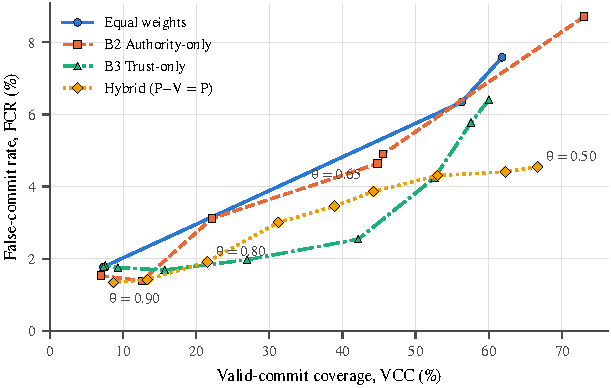
\includegraphics{fig2_threshold_tradeoff.pdf}
\caption{Commit-threshold trade-off after Revenue degrades (S2): false-commit rate against valid-commit coverage as $\theta$ varies from 0.50 to 0.90 in steps of 0.05 (means over 100 seeds, ideal feedback)}
\label{fig:threshold}
\end{figure}
% Auto-generated by paper_assets/build_assets.py from saved results -- do not edit numbers by hand.
% Preamble needs: \usepackage{booktabs,array,tabularx,makecell}
\begin{table}[tb]
\centering
\caption{Exploratory robustness study A2: levels at which each main conclusion holds, with the range of FCR differences in points}\label{tab:robustness}
\footnotesize
\setlength{\tabcolsep}{3pt}
\renewcommand{\arraystretch}{1.1}
\begin{tabularx}{\textwidth}{@{}>{\raggedright\arraybackslash}Xcccc@{}}
\toprule
Factor varied & C1 (S1) & C1 (S2) & C2 & C3 \\
\midrule
Off-home accuracy 0.60--0.85 & \makecell{4/4 \\ ($-$6.2 to $-$0.4)} & \makecell{4/4 \\ ($-$4.9 to $-$1.4)} & \makecell{3/4 \\ ($-$1.6 to $-$0.2)} & \makecell{4/4 \\ ($-$1.3 to $-$0.8)} \\
Home accuracy 0.85--0.95 & \makecell{3/3 \\ ($-$2.0 to $-$0.9)} & \makecell{3/3 \\ ($-$2.5 to $-$1.6)} & \makecell{3/3 \\ ($-$1.3 to $-$1.1)} & \makecell{3/3 \\ ($-$1.9 to $-$1.3)} \\
Shared R+S errors $\rho$ = 0--0.20 & \makecell{4/4 \\ ($-$3.6 to $-$2.0)} & \makecell{4/4 \\ ($-$3.6 to $-$2.5)} & \makecell{4/4 \\ ($-$2.0 to $-$1.3)} & \makecell{4/4 \\ ($-$5.0 to $-$1.3)} \\
Label noise e = 0--0.10, F0 & --- & \makecell{4/4 \\ ($-$2.5 to $-$2.4)} & \makecell{4/4 \\ ($-$1.3 to $-$1.1)} & \makecell{4/4 \\ ($-$1.3 to $-$1.2)} \\
Label noise e = 0--0.10, F1 & --- & \makecell{4/4 \\ ($-$2.6 to $-$2.5)} & \makecell{4/4 \\ ($-$1.6 to $-$1.4)} & \makecell{4/4 \\ ($-$0.9 to $-$0.8)} \\
\bottomrule
\end{tabularx}
\par\smallskip
\parbox{\textwidth}{\scriptsize C1: hybrid below majority. C2: hybrid below authority-only after degradation (requests 251--1000). C3: trust-only below hybrid (S2). Holds: the 95\% CI excludes 0 with the main-study sign. No conclusion reversed.}
\end{table}

\begin{figure}[tb]
\centering
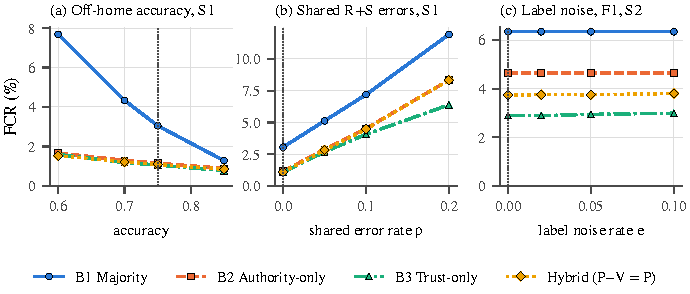
\includegraphics{fig3_robustness.pdf}
\caption{Exploratory robustness study A2 (100 seeds): false-commit rate by mechanism as (a) off-home accuracy, (b) the shared error rate of Revenue and Sub-Registrar and (c) label noise vary; dotted lines mark the main-study settings}
\label{fig:robustness}
\end{figure}
\clearpage
\section*{Supplementary material (Fig. S1, Tables S1--S4)}
\setcounter{table}{0}\setcounter{figure}{0}
\renewcommand{\thetable}{S\arabic{table}}
\renewcommand{\thefigure}{S\arabic{figure}}
% Auto-generated by paper_assets/build_assets.py from saved results -- do not edit numbers by hand.
% Preamble needs: \usepackage{booktabs,array,tabularx,makecell}
\begin{table}[tb]
\centering
\caption{Illustrative meaning of each simulated report (+1 / $-$1; $\varnothing$ = no response)}\label{tab:normalisation}
\footnotesize
\setlength{\tabcolsep}{3pt}
\renewcommand{\arraystretch}{1.1}
\begin{tabularx}{\textwidth}{@{}>{\raggedright\arraybackslash}p{1.5cm}*{3}{>{\raggedright\arraybackslash}X}@{}}
\toprule
Office & own: seller is recorded holder & deed: deed registered, matching & restr: no pending proceeding \\
\midrule
Revenue & Home. +1 record of rights names the seller; $-$1 names another & +1 mutation file cites a matching deed; $-$1 no match & +1 no pending revenue proceeding noted; $-$1 one is noted \\
Sub-Registrar & +1 earlier registered documents consistent with seller; $-$1 not & Home. +1 deed registered, parties and parcel match; $-$1 not & +1 no notice of a pending suit noted; $-$1 one is noted \\
Judiciary & +1 no court record contradicts the holding; $-$1 a decree names another holder & +1 no case challenges the deed; $-$1 one does & Home. +1 nothing pending in any forum covered; $-$1 a proceeding is pending \\
\bottomrule
\end{tabularx}
\par\smallskip
\parbox{\textwidth}{\scriptsize Simulated signals only; not claims about the records real offices hold or certify.}
\end{table}

% Auto-generated by paper_assets/build_assets.py from saved results -- do not edit numbers by hand.
% Preamble needs: \usepackage{booktabs,array,tabularx,makecell}
\begin{table}[tb]
\centering
\caption{Exploratory coverage-gate ablation A1 (paired 95\% CIs, 100 seeds, percentage points)}\label{tab:ablation}
\footnotesize
\setlength{\tabcolsep}{3pt}
\renewcommand{\arraystretch}{1.1}
\begin{tabularx}{\textwidth}{@{}>{\raggedright\arraybackslash}Xccc@{}}
\toprule
Comparison & Scenario & FCR difference & VCC difference \\
\midrule
Hybrid $-$ majority, no gate (G0) & S1 & $-$1.85 [$-$2.00, $-$1.69] & $-$0.27 [$-$0.53, $-$0.004] \\
Hybrid $-$ majority, no gate (G0) & S4 & $-$0.99 [$-$1.14, $-$0.83] & +8.41 [+8.13, +8.70] \\
Hybrid $-$ majority, common count gate (G1) & S1 & $-$1.85 [$-$2.01, $-$1.70] & $-$0.27 [$-$0.53, $-$0.004] \\
Hybrid $-$ majority, common count gate (G1) & S4 & $-$1.01 [$-$1.19, $-$0.83] & +8.41 [+8.13, +8.70] \\
Hybrid: weighted gate $-$ count gate & S1 & $-$0.11 [$-$0.15, $-$0.07] & $-$4.25 [$-$4.39, $-$4.11] \\
Hybrid: weighted gate $-$ count gate & S4 & $-$0.72 [$-$0.85, $-$0.60] & $-$21.23 [$-$21.52, $-$20.95] \\
\bottomrule
\end{tabularx}
\end{table}

\begin{figure}[tb]
\centering
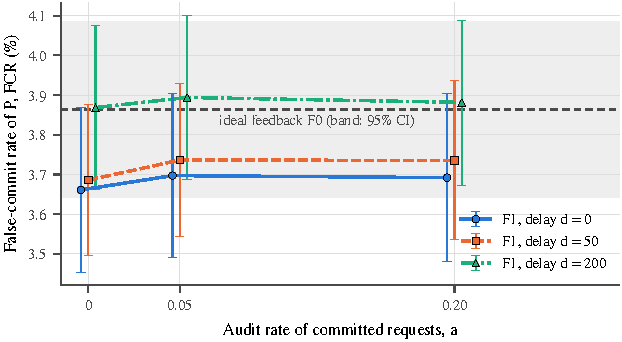
\includegraphics{figS1_feedback.pdf}
\caption{False-commit rate of P under realistic feedback F1 in S2, by audit rate and label delay; whiskers are between-seed 95\% CIs, the dashed line and band show ideal feedback F0}
\label{fig:feedback}
\end{figure}
\clearpage
% Auto-generated by paper_assets/build_assets.py from saved results -- do not edit numbers by hand.
% Preamble needs: \usepackage{booktabs,array,tabularx,makecell}
\begin{table}[tb]
\centering
\caption{Status of every result}\label{tab:status}
\footnotesize
\setlength{\tabcolsep}{3pt}
\renewcommand{\arraystretch}{1.1}
\begin{tabularx}{\textwidth}{@{}>{\raggedright\arraybackslash}p{4.8cm}>{\raggedright\arraybackslash}X@{}}
\toprule
Result & Status \\
\midrule
Tables 6--7; Fig. 2; Fig. S1; $q_{\min}$ sweep & Pre-specified (frozen protocol); five analysis choices in Table S4 \\
Veto bound (Sect. 3) & Analytic, derived before the protocol freeze \\
Counts per 1,000 requests; quoted trust values & Descriptive re-expression of pre-specified runs \\
Two-sided test for H5 & Exploratory, added after results were seen \\
Table S2 (A1); Table 8 and Fig. 3 (A2) & Exploratory; addenda committed before running \\
\bottomrule
\end{tabularx}
\end{table}

% Auto-generated by paper_assets/build_assets.py from saved results -- do not edit numbers by hand.
% Preamble needs: \usepackage{booktabs,array,tabularx,makecell}
\begin{table}[tb]
\centering
\caption{Analysis choices not covered by the frozen protocol (accepted by the supervisor)}\label{tab:notes}
\footnotesize
\setlength{\tabcolsep}{3pt}
\renewcommand{\arraystretch}{1.1}
\begin{tabularx}{\textwidth}{@{}c>{\raggedright\arraybackslash}p{4.2cm}>{\raggedright\arraybackslash}X@{}}
\toprule
\# & Situation & Choice \\
\midrule
1 & H4 has zero variance & Interval is the point 0; p = 1.0 in the Holm family \\
2 & H1b has no direction & Two-sided test inside the Holm family of seven \\
3 & Significant and inside $\pm$$\Delta$ (H1b) & Worded `lower, but smaller than $\Delta$' \\
4 & CI opposite a one-sided hypothesis (H5) & `Not supported'; two-sided CI and exploratory test reported \\
5 & H3 has no direction & Worded from its unadjusted CI; labelled descriptive \\
\bottomrule
\end{tabularx}
\end{table}

\end{document}
